\chapter{Deep Declarative Network}
\label{cha:ddn}
In this chapter, we will cover the structure and nodes in the deep declarative network: from its learning process to the back-propagation.
\par Before delving into the details of the back-propagation in different constraints cases, we give an overview of the deep declarative network in Section~\ref{sec:overview-ddn}. In particular, the basic structure of the network and the details of declarative nodes are described according to \cite{SG:19}. The learning progress of the network is also given. We hope this will give readers a better sense of what is the deep declarative network and how it works. 
\par In Section~\ref{sec:bp}, we present the details of the back-propagation in different constrained problems. The gradient computation results are based on the implicit differentiation and different in constrained problems. We discuss this part based on the regular solution and compare it with the general solution in the previous chapter. 
\par Next we present the examples of constrained optimization problems with both linear and non-linear, equality and inequality constraints in Section~\ref{sec:example}. We also provide more implementation details of the deep declarative nodes. 
\par Finally, we summarize the deep declarative network and its solution in different constrained problems under the regular point. 


\section{An Overview of Deep Declarative Network}
\label{sec:overview-ddn}
\subsection{Declarative Node}
In deep declarative network, it defines the solution of a constrained optimization problem with parameter $x \in \mathbb{R}^n$ as the output of each node $y \in \mathbb{R}^m$. The general optimization problem can be defined as 
\begin{equation}
    \label{equ:ddn-basic}
    y \in \underset{u \in C}{\arg \min } f(x, u)
\end{equation}
where $f$ is the objective function $f: \mathbb{R}^n \times \mathbb{R}^m \rightarrow \mathbb{R}$, and $C \in \mathbb{R}^m$ is the set of constraints parameterized by $x$. 
\par Apart from the traditional forward processing mapping node, deep declarative node does not explicitly define the transforming function from the input to the output. It defines the input-output relationship implicitly by an objective and constraints optimization problem, where the solution of the problem is the output. 
\begin{figure}
    \label{fig:ddn}
    \centering
    \tikzset{every picture/.style={line width=0.75pt}} %set default line width to 0.75pt        

    \begin{tikzpicture}[x=0.75pt,y=0.75pt,yscale=-1,xscale=1]
    %uncomment if require: \path (0,300); %set diagram left start at 0, and has height of 300

    %Rounded Rect [id:dp5847695584847934] 
    \draw   (233,118.5) .. controls (233,113.81) and (236.81,110) .. (241.5,110) -- (421,110) .. controls (425.69,110) and (429.5,113.81) .. (429.5,118.5) -- (429.5,177.14) .. controls (429.5,181.84) and (425.69,185.64) .. (421,185.64) -- (241.5,185.64) .. controls (236.81,185.64) and (233,181.84) .. (233,177.14) -- cycle ;
    %Straight Lines [id:da8797940676718146] 
    \draw    (197.5,135.64) -- (230.5,135.64) ;
    \draw [shift={(232.5,135.64)}, rotate = 180] [color={rgb, 255:red, 0; green, 0; blue, 0 }  ][line width=0.75]    (10.93,-3.29) .. controls (6.95,-1.4) and (3.31,-0.3) .. (0,0) .. controls (3.31,0.3) and (6.95,1.4) .. (10.93,3.29)   ;
    %Straight Lines [id:da5288114309680509] 
    \draw    (232.5,165.64) -- (200.5,165.64) ;
    \draw [shift={(198.5,165.64)}, rotate = 360] [color={rgb, 255:red, 0; green, 0; blue, 0 }  ][line width=0.75]    (10.93,-3.29) .. controls (6.95,-1.4) and (3.31,-0.3) .. (0,0) .. controls (3.31,0.3) and (6.95,1.4) .. (10.93,3.29)   ;
    %Straight Lines [id:da8485926924080154] 
    \draw    (429.5,135.64) -- (462.5,135.64) ;
    \draw [shift={(464.5,135.64)}, rotate = 180] [color={rgb, 255:red, 0; green, 0; blue, 0 }  ][line width=0.75]    (10.93,-3.29) .. controls (6.95,-1.4) and (3.31,-0.3) .. (0,0) .. controls (3.31,0.3) and (6.95,1.4) .. (10.93,3.29)   ;
    %Straight Lines [id:da8644978866807145] 
    \draw    (463.5,165.64) -- (431.5,165.64) ;
    \draw [shift={(429.5,165.64)}, rotate = 360] [color={rgb, 255:red, 0; green, 0; blue, 0 }  ][line width=0.75]    (10.93,-3.29) .. controls (6.95,-1.4) and (3.31,-0.3) .. (0,0) .. controls (3.31,0.3) and (6.95,1.4) .. (10.93,3.29)   ;
    %Straight Lines [id:da03877231252818136] 
    \draw    (300,78.5) -- (300,107.64) ;
    \draw [shift={(300,109.64)}, rotate = 270] [color={rgb, 255:red, 0; green, 0; blue, 0 }  ][line width=0.75]    (10.93,-3.29) .. controls (6.95,-1.4) and (3.31,-0.3) .. (0,0) .. controls (3.31,0.3) and (6.95,1.4) .. (10.93,3.29)   ;
    %Straight Lines [id:da34598442566525556] 
    \draw    (350,109.64) -- (350,80.64) ;
    \draw [shift={(350,78.64)}, rotate = 450] [color={rgb, 255:red, 0; green, 0; blue, 0 }  ][line width=0.75]    (10.93,-3.29) .. controls (6.95,-1.4) and (3.31,-0.3) .. (0,0) .. controls (3.31,0.3) and (6.95,1.4) .. (10.93,3.29)   ;

    % Text Node
    \draw (260,140) node [anchor=north west][inner sep=0.75pt]   [align=left] {$\displaystyle y\ \in \underset{u\ \in \ C}{\arg\min} f( x,\ u;\ \theta ) \ $};
    % Text Node
    \draw (175,130) node [anchor=north west][inner sep=0.75pt]   [align=left] {$\displaystyle x$};
    % Text Node
    \draw (145,158) node [anchor=north west][inner sep=0.75pt]   [align=left] {$\displaystyle \operatorname{D} J( x)$};
    % Text Node
    \draw (475,130) node [anchor=north west][inner sep=0.75pt]   [align=left] {$\displaystyle y$};
    % Text Node
    \draw (472,158) node [anchor=north west][inner sep=0.75pt]   [align=left] {$\displaystyle \operatorname{D} J( y)$};
    % Text Node
    \draw (295,58) node [anchor=north west][inner sep=0.75pt]   [align=left] {$\displaystyle \theta $};
    % Text Node
    \draw (332,55) node [anchor=north west][inner sep=0.75pt]   [align=left] {$\displaystyle \operatorname{D} J( \theta )$};
    \end{tikzpicture}

    \caption{End-to-end learnable declarative node}
\end{figure}
\par Figure~\ref{fig:ddn} shows the forward and backward pass of the declarative node. In the forward evaluation pass, the output of the declarative $y$ is computed as the solution of some minimization problem $f(x, u; \theta)$. We use $\operatorname{D}$ to denote the total derivative with respect to the independent variables. Therefore, in the backward pass, the gradient of the global objective function with respect to the output $\operatorname{D}J(y)$ is back-propagated. Its value is computed through the chain rule based on the gradients with respect to the input $\operatorname{D}J(x)$ and parameters $\operatorname{D}J(\theta)$.
\par Since the definition of deep declarative nodes is very general, it can be embedded within another network for solving subproblems such as robust fitting. However, we may not be able to find the gradient when the feasible set is discrete, or the declarative node is low efficiency to evaluate. As non-regular solution cases, the nonexistent gradient problem will be discussed in the next part. In the next subsection, the learning details of the deep declarative network are described. 

\subsection{Learning}
Since in declarative nodes, there is no explicit forward function defined, we can directly compute the optimal solution $y$ through some algorithms. Under this assumption, when we performing the back-propagation, we can compute the gradient of the output from each node with respect to the corresponding input through the implicit differentiation directly. This can be treated as a bi-level optimization problem\citep{BJ:98} where the parameterized constraints as a lower-level problem blinds variables in the objective function, an upper-level problem. Combining the schematic illustration in Figure~\ref{fig:ddn}, the problem can be defined formally as
\begin{equation}
    \begin{array}{ll}\operatorname{minimize} & J(x, y) \\ \text { subject to } & y \in \arg \min _{u \in C} f(x, u)\end{array}
\end{equation}
\par We may have additional layers to make the objective function $J(x, y)$ depend on $y$, which is a function of $x$. In general, it is the sum of loss terms and regularization terms. We can solve this minimization problem through the gradient descent as follows:
\begin{equation}
    \operatorname{D}J(x,y) = \operatorname{D}_XJ(x,y) + \operatorname{D}_YJ(x,y)\operatorname{D}y(x)
\end{equation}
where $\operatorname{D}_XJ(x,y)$ is the partial derivatives of $J(x,y)$ with respect to $x$ and $\operatorname{D}_YJ(x,y)$ is the partial derivatives of $J(x,y)$ with respect to $y$. We used to use $\operatorname{D}_X$ and $\operatorname{D}_Y$ to denote the partial derivatives. We decompose the total derivatives of $J(x,y)$ as the sum of the partial derivatives with the chain rule. In application, we can consider it as the sum of gradients for losses on training examples. 
\par The lower-level objective function $f$ can be simpler. If it is the only term involving $y$ in the upper-level objective function $J$, that means $J(x,y) = g(x, f(x,y))$ and the lower-level problem is actually unconstrained with $u \in C=\mathbb{R}^m$. Under this condition, the calculation of the gradient can be expanded using chain rule through both $\operatorname{D}_XJ(x,y)$ and $\operatorname{D}_YJ(x,y)$:
\begin{equation}
    \begin{aligned} 
        \operatorname{D} J(x, y) &=\operatorname{D}_{X} g(x, f)+\operatorname{D}_{F} g(x, f)\left(\operatorname{D} f+\operatorname{D}_{Y} f \operatorname{D} y\right) \\ &=\operatorname{D}_{X} g(x, f)+\operatorname{D}_{F} g(x, f) \operatorname{D} f 
    \end{aligned}
\end{equation}
where $\operatorname{D}_Yf(x,y) = 0$ since $y$ is the minimum of $f(x,y)$ and $f(x,y)$ is an unconstrained problem, its partial derivative should be zero. 
\par In addition, for the solution $y$, we should verify its regularity. 
\begin{defn}[Regular Point]~\citep{SG:19}
    A feasible point $u$ is said to be \emph{regular} if the equality constraints gradient $D_Uh_i$ and the active inequality constraints gradients $D_Ug_i$ are linearly independent, or there are no equality constraints and the inequality constraints are all inactive at $u$.
\end{defn}
Therefore, in unconstrained problems, we can consider the solution is regular by default. However in constrained problems, especially the inequality constrained problems, we should be aware of the feasible set is continuous or not. 

\section{Back-propagation Through Declarative Nodes}
\label{sec:bp}
Let us focus back on the more general case with $y$ involving in different terms. The backward pass is different in different sub-classes of declarative nodes. We consider three common cases based on Equation~\ref{equ:ddn-basic}. 

\subsection{Unconstrained}
Firstly, the most basic case is the unconstrained problem. Consider a function $f: \mathbb{R}^n \times \mathbb{R}^m \rightarrow \mathbb{R}$, we have
\begin{equation}
    y \in \underset{u \in C}{\arg \min } f(x, u)
\end{equation}
\par We make the assumption that the solution of this problem, $y(x)$ exists, and in the neighborhood of the point $(x, y(x))$, $f$ is second-order differentiable. Therefore, we can compute the derivative of $y$ with respect to $x$ is
$$
\operatorname{D}y(x) = -H^{-1}B
$$
where $H = \operatorname{D}_{YY}^2 f(x, y(x)) \in \mathbb{R}^{m \times m}$ is the second-order derivative of $f$ with respect to $y$, and it is a non-singular matrix. $B = \operatorname{D}_{XY}^2 f(x, y(x)) \in \mathbb{R}^{m \times n}$ is the second-order derivative of $f$ with respect to $y$ and $x$ (the derivative of $D_Yf(x,y)$ with respect to $x$). 
\par The proof of this solution is similar to the proof of Equation~\ref{equ:2.3}: setting the partial derivative of $f(x,y)$ with respect to the optimal $y$ as 0, then transposing and differentiating both sides according to the implicit function theorem: 
\begin{equation}
    \begin{aligned} 
        0_{m \times n} &=\operatorname{D}\left(\operatorname{D}_{Y} f(x, y)\right)^{T} \\ &=\operatorname{D}_{X Y}^{2} f(x, y)+\operatorname{D}_{Y Y}^{2} f(x, y) \operatorname{D} y(x) 
    \end{aligned}
\end{equation}
After rearrangement, we get
\begin{equation}
    \operatorname{D} y(x)=-\left(\operatorname{D}_{Y Y}^{2} f(x, y)\right)^{-1} \operatorname{D}_{X Y}^{2} f(x, y)
\end{equation}
\par Since this is the unconstrained case, for any stationary point of $f(x,y)$, the result is valid. In the following constrained cases, the optimal solution is actually the stationary point of the Lagrangian. 

\subsection{Equality Constrained}
Secondly, we consider the equality constrained problem, that means the feasible set is defined by $p$ nonlinear equality constraints. Consider functions $f: \mathbb{R}^n \times \mathbb{R}^m \rightarrow \mathbb{R}$ and $h: \mathbb{R}^n \times \mathbb{R}^m \rightarrow \mathbb{R}^p$, we have
\begin{equation}
    \begin{aligned} 
        y(x) \in & \arg \min _{u \in \mathbb{R}^{m}} f(x, u) \\ & \text { subject to } \quad h_{i}(x, u)=0, i=1, \ldots, p 
    \end{aligned}
\end{equation}
where $h = [h_1, \dots, h_p]^T$ are a set of constraints. 
\par Again, we make the assumption that the solution of this problem, $y(x)$ exists and both $f$ and all constraints in $h$ are second-order differentiable. Also, we should consider the Jacobian matrix of $h$ with respect to $y$ is full rank since we need the optimal point is regular. Then we can calculate the derivative of $y$ with respect to $x$ is
$$
\operatorname{D} y(x)=H^{-1} A^{T}\left(A H^{-1} A^{T}\right)^{-1}\left(A H^{-1} B-C\right)-H^{-1} B
$$
where
$$
\begin{aligned} 
    A &=\operatorname{D}_{Y} h(x, y) \in \mathbb{R}^{p \times m} \\ B &=\operatorname{D}_{X Y}^{2} f(x, y)-\sum_{i=1}^{p} \lambda_{i} \operatorname{D}_{X Y}^{2} h_{i}(x, y) \in \mathbb{R}^{m \times n} \\ C &=\operatorname{D}_{X} h(x, y) \in \mathbb{R}^{p \times n} \\ H &=\operatorname{D}_{Y Y}^{2} f(x, y)-\sum_{i=1}^{p} \lambda_{i} \operatorname{D}_{Y Y}^{2} h_{i}(x, y) \in \mathbb{R}^{m \times m} 
\end{aligned}
$$
and $\lambda \in \mathbb{R}^p$ can be solved through the system $\lambda ^T A = \operatorname{D}_Yf(x,y)$. 
\par Similar to the solution of linear equality constrained problem in Equation~\ref{equ:2.4}, we can form the Lagrangian by the method of Lagrange multipliers\citep{BD:14}:
\begin{equation}
    \mathcal{L}(x, y, \lambda)=f(x, y)-\sum_{i=1}^{p} \lambda_{i} h_{i}(x, y)
\end{equation}
\par We introduce the Lagrange multipliers $\lambda$ to set the stationary point of this Lagrangian is $(y, \lambda)$. Then we differentiate $\mathcal{L}$ with respect to $y$ and $\lambda$ separately, which are both resulting in 0 since $y$ is the optimality. We have two cases at the optimal point $y$. The first one is that the partial derivatives of $f$ with respect to $y$ equals to zero: $\operatorname{D}_Yf(x,y) = 0 \in \mathbb{R}^{1 \times m}$. That means we transfer this problem to an unconstrained problem since its solution satisfies the constraints directly. Under this case, $\lambda$ can be set as 0 directly. The second one is that the partial derivatives of $f$ with respect to $y$ is non-zero vector, and it is orthogonal to the constraint surface, which is controlled by the set of equality constraints $h(x, y) = 0$. In this case, from the derivative of $\mathcal{L}$ with respect to $y$ equaling to zero, we have
\begin{equation}
    \mathrm{D}_{Y} f(x, y)=\sum_{i=1}^{p} \lambda_{i} \mathrm{D}_{Y} h_{i}(x, y)=\lambda^{T} A
\end{equation}
where $A$ is the same as the defined above. 
\par To solve this equation for $\lambda$, if we want to compute explicitly, it has a unique analytic solution $\lambda = (AA^T)^{-1}A(\operatorname{D}_Yf)^T$. 

\par Next, we compute the second-order derivative of $\mathcal{L}$ with respect to $x$. It still equals to zero in both functions. Solving the equation through variable elimination~\citep{BS:04} we have
\begin{equation}
    \operatorname{D} \lambda(x)=\left(A H^{-1} A^{T}\right)^{-1}\left(A H^{-1} B-C\right)
\end{equation}

\begin{equation}
    \operatorname{D} y(x)=H^{-1} A^{T}\left(A H^{-1} A^{T}\right)^{-1}\left(A H^{-1} B-C\right)-H^{-1} B
\end{equation}
which is our result. 
\par The problem and solution defined in Section~\ref{sec:equ-opt} is the simplier case of this general one. Also, if we only have one constraint, the matrix $A$ and vector $\lambda$ can be simplifed as vector and scalar separately. Moreover, for linear only constraints, the repsentation of matrix $H$ and $B$ are also simper since $\lambda = 0$.  

\subsection{Inequatlity Constrained}
Lastly, inequality constrained problems are more complicated since we have to consider the solution for active and inactive constraints. Also, previous works metioned in Section~\ref{sec:ineq-opt} are approximation results or focusing on the convex problems. Here, the declarative nodes consider the the problem containing both equality and inequality constraints. Consider functions $f: \mathbb{R}^n \times \mathbb{R}^m \rightarrow \mathbb{R}$ and $h: \mathbb{R}^n \times \mathbb{R}^m \rightarrow \mathbb{R}^p$, and $g: \mathbb{R}^n \times \mathbb{R}^m \rightarrow \mathbb{R}^q$, we have
\begin{equation}
    \begin{aligned} 
        y(x) \in & \arg \min _{u \in \mathbb{R}^{m}} f(x, u) \\ & \text { subject to } \quad\begin{array}{l}h_{i}(x, u)=0, i=1, \ldots, p \\ g_{i}(x, u) \leq 0, i=1, \ldots, q\end{array}
    \end{aligned}
\end{equation}
where $h = [h_1, \dots, h_p]^T$ are still a set of equality constraints, and $g = [g_1, \dots, g_q]^T$ are a set of inequality constraints. 
\par In declarative nodes, it present a more general result based on activity of all inequality constraints at the optimal point $y(x)$. Also, assumptions of the existence of the optimal point $y(x)$ and second-order differentiation of $f$, $g$, $h$ remain true. We combine the equality constraints and inequality constraints together in $\tilde{h} = [h_1, \dots, h_p, g_1, \dots, g_q]$ and the derivative of $\tilde{h}$ with respect to $y$ is a full rank matrix to keep the regularity. We have
$$
\operatorname{D} y(x)=H^{-1} A^{T}\left(A H^{-1} A^{T}\right)^{-1}\left(A H^{-1} B-C\right)-H^{-1} B
$$
where
$$
\begin{aligned} 
    A &=\operatorname{D}_{Y} \tilde{h}(x, y) \in \mathbb{R}^{(p+q) \times m} \\ B &=\operatorname{D}_{X Y}^{2} f(x, y)-\sum_{i=1}^{p} \lambda_{i} \operatorname{D}_{X Y}^{2} \tilde{h}_{i}(x, y) \in \mathbb{R}^{m \times n} \\ C &=\operatorname{D}_{X} \tilde{h}(x, y) \in \mathbb{R}^{(p+q) \times n} \\ H &=\operatorname{D}_{Y Y}^{2} f(x, y)-\sum_{i=1}^{p+q} \lambda_{i} \operatorname{D}_{Y Y}^{2} \tilde{h}_{i}(x, y) \in \mathbb{R}^{m \times m} 
\end{aligned}
$$
and $\lambda \in \mathbb{R}^{p+q}$ satisfies $\lambda ^T A = \operatorname{D}_Yf(x,y)$ with $\lambda_i \leq 0$ for $i = p+1, \dots, p+q$, which is almost the same as the solution of the equality constrained problem. 
\par However, in inequality constraints, the gradient is discontinuous since the Lagrange multipliers $\lambda$ for active inequality constraints are zero. We separate the solution of inequality constrained declarative nodes into 3 scenarios. For any inequality constraints $g(x, u) \leq 0$, the constraint can be active or inactive at the optimal solution $y$. In the first scenario, the constraint is inactive at the solution $y$, that means $g(x,y) < 0$ and it is completely in the feasible set. Therefore we have $\operatorname{D}_Yf(x,y) = 0$ and we can consider it as an unconstrained problem. In the second scenario, the constraint is active at $y$, but it is orthogonal to the constraint surface. Then we have $\operatorname{D}_Yf(x,y) \neq 0$ and $\lambda \neq 0$. Then we can consider this inequality constraint as an equality one since the solution falls on the boundary of the feasible set, but the gradient of negative and pointing outside the set. The last scenario, the constraint is active and $\operatorname{D}_Yf(x,y) = 0$ when the solution is on the boundary and it is a local minimum. For the backward propagation, in this case, we can choose both solutions of unconstrained or equality constrained gradient. 

\section{Examples of Declarative Nodes}
\label{sec:example}
\subsection{Implementation Details}
We give the implementation of both equality and inequality constraints with linear and nonlinear cases in raw Python under the gradient calculation package Autograd\citep{MD:15}. In this subsection, we are going to show the implementation details of the basic deep declarative nodes.
\par \textbf{Constraints definition.}  
In the multiple equality constraints node and inequality constraints node, equality constraints and inequality constraints are defined in two functions separately. If there are more than one constraint, they are stored in a 1-d array. All constraints equal to zero or less than 0, which means all parameters in the equations are in the left-hand side and the right-hand side is always zero. There is a specific checking function defined to check this. In the linear equality constraints node, the set of linear constraints are defined as a single matrix $A$ and its corresponding vector $b$ in the initialization directly. 

\par \textbf{Gradient computation.}
To compute the gradient of the solution under the constraints, we need to calculate the Jacobian and Hessian matrix, which are the first-order and second-order derivative matrix of the constraints. For matrix $H$ in the general solution of the constrained problem, it is costly to compute the inverse of it. Therefore, we transfer the problem to solving a linear system $Hx_1 = A^T$ and $Hx_2 = B$ where $x_1 = H^{-1}A^T$ and $x_2 = H^{-1}B$ to solve them. Cholesky decomposition, an algorithm for solving the linear system efficiently, is applied to this problem. It decomposes a Hermitian positive-definite matrix into the product of a lower triangular matrix with real and positive diagonal entries with its conjugate transpose, which is the unique decomposition. In our problems, since matrix $H$ is a symmetric real positive-definite matrix, it can be decomposed through this algorithm effectively. The solution of the Lagrange multipliers $\lambda$ similar, which is the solution of a linear system $\lambda^T A = \operatorname{D}_Yf(x,y)$ through the least-square solution solver. 
\par \textbf{Optimality checking.} For constrained optimization problems, according to the optimality conditions defined in Section~\ref{sec:opt-con-constrained}, we should check if the first-order optimality condition is satisfied or not. We define a function in all cases for checking the optimality: the gradient of constraint is zero at optimal point ($\operatorname{D}_Yh(x,y) = 0$), or the gradient of objective function equals to the product of the Lagrange multipliers and the gradient of constraints ($\operatorname{D}_Yf(x, y) = \lambda \operatorname{D}_Yh(x, y)$). 

\par \textbf{Exception handling.}
Since our assumptions are based on the regular solution, and not all problems have a regular optimal point, we define the exception cases for this problem. When we solve the linear system for the Lagrange multipliers $\lambda$, if the solution does not falls as a regular point, we may get a null value in $\lambda$ due to the non-existence of the gradient on a non-regular solution. We are going to discuss the solution for this specific case in the next part. For here, we just throw the exception once there is a null value in the Lagrange multipliers $\lambda$. 

\subsection{Equality Constrained}
Firstly, we consider a single linear equality constrained problem, minimizing the KL-divergence between the input $x$ and output $y$ subject to the output forming a valid probablility vector, which can be formally defined as 
\begin{equation}
    \begin{array}{rll}
        y =& \text{argmin}_u & - \sum_{i=1}^{n} x_i \log u_i \\
        & \text{subject to} & \sum_{i=1}^{n} u_i = 1
    \end{array}
\end{equation}
where the positivity constraint on $y$ is automatically satisfied by the domain of the log function.
\begin{figure}[t]
    \label{fig:equ-lin-eg}
    \centering
    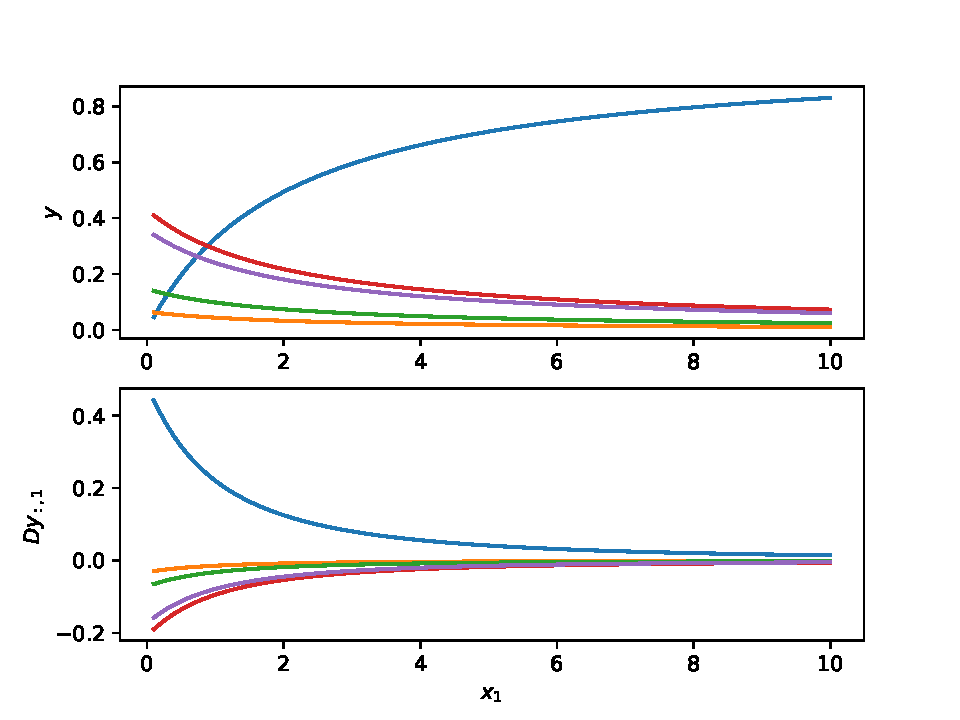
\includegraphics[page=1,width=.8\textwidth]{figs/linear_equality_example.pdf} 
    \caption{Plots of the function $y$ (top) and the gradient (bottom) sweeping the first component of the input $x_1$ while holding the other elements of $x$ constant}
\end{figure}
\par A nice feature of this problem is that we can solve it in closed-form as
$$
y = \frac{1}{\sum_{i=1}^{n} x_i} x.
$$

\par Now we are going to solve this problem via an iterative method with derivative of deep declarative node. Set $n=5$ and $m=5$, which means the input $x \in \mathbb{R}^5$ and the output $y \in \mathbb{R}^5$. We begin from a random feasible solution, which is the normalization of the value $y$, then preform the gradient update. Figure~\ref{fig:equ-lin-eg} shows the function and gradient sweeping the first component of the input $x_1$ from 0.1 to 10.0 while holding the other elements of $x$ constant. 
\par Now we consider a multiple non-linear equality constrained problem which is defined formally as
\begin{equation}
    \begin{array}{rll}
        y =& \text{argmin}_u & \sum_{i=1}^{n} x_i u_i^{2} \\
        & \text{subject to} & \sum_{i=1}^{n-1} u_i^2 = 1 \\
        & & \sum_{i=1}^{n} u_i = 0 \\
    \end{array}
\end{equation}
\begin{figure}[t]
    \label{fig:equ-nonlin-eg}
    \centering
    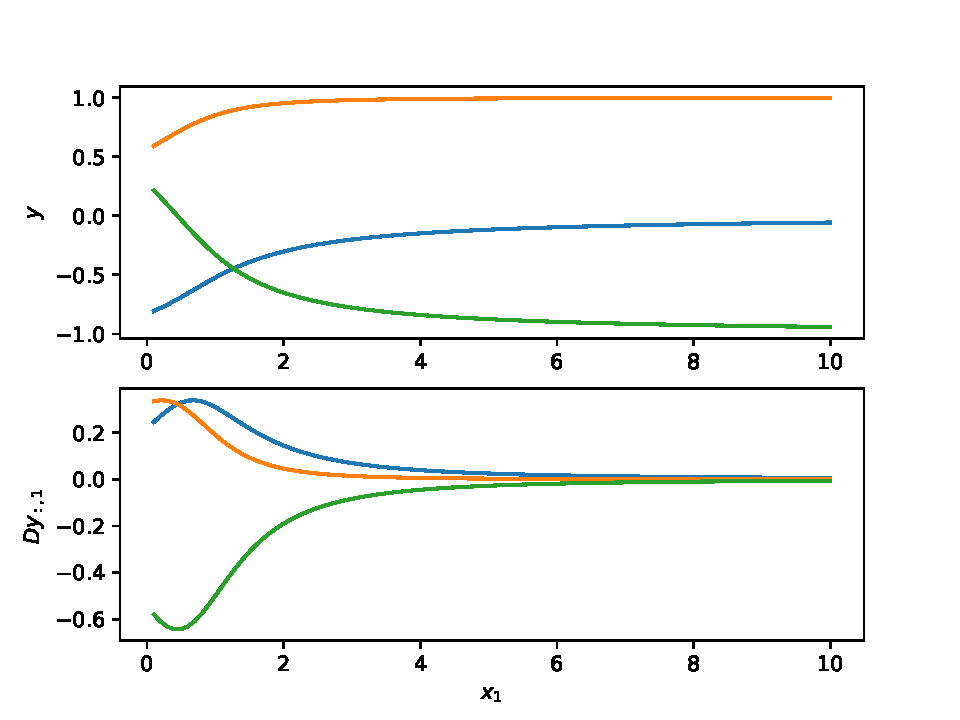
\includegraphics[page=1,width=.8\textwidth]{figs/multiple_equality_example.pdf} 
    \caption{Plots of the function $y$ (top) and the gradient (bottom) sweeping the first component of the input $x_1$ while holding the other elements of $x$ constant}
\end{figure}
\par Same as the previous example, we instantiate the multiple equality constriants nodes in deep declarative nodes with $n=3$ and $m=3$. We begin from a feasible solution, $\cos^2 x + \sin^2 x - \sin x - \cos x = 0$, performing the gradient descent until the convergence. Figure~\ref{fig:equ-nonlin-eg} shows the function $y$ and its gradient changes. 
\subsection{Inequatlity Constrained}
For inequality constrained problems, we consider a similar problem based on the multiple equality constrained problem above. The only difference is that we restrict the first parameter $u_1$ is less than $u_2$. Therefore, the problem is defined as
\begin{equation}
    \begin{array}{rll}
        y =& \text{argmin}_u & \sum_{i=1}^{n} x_i u_i^{2} \\
        & \text{subject to} & \sum_{i=1}^{n-1} u_i^2 = 1 \\
        & & \sum_{i=1}^{n} u_i = 0 \\
        & & u_1 - u_2 < 0
    \end{array}
\end{equation}
\begin{figure}[t]
    \label{fig:ineq-eg}
    \centering
    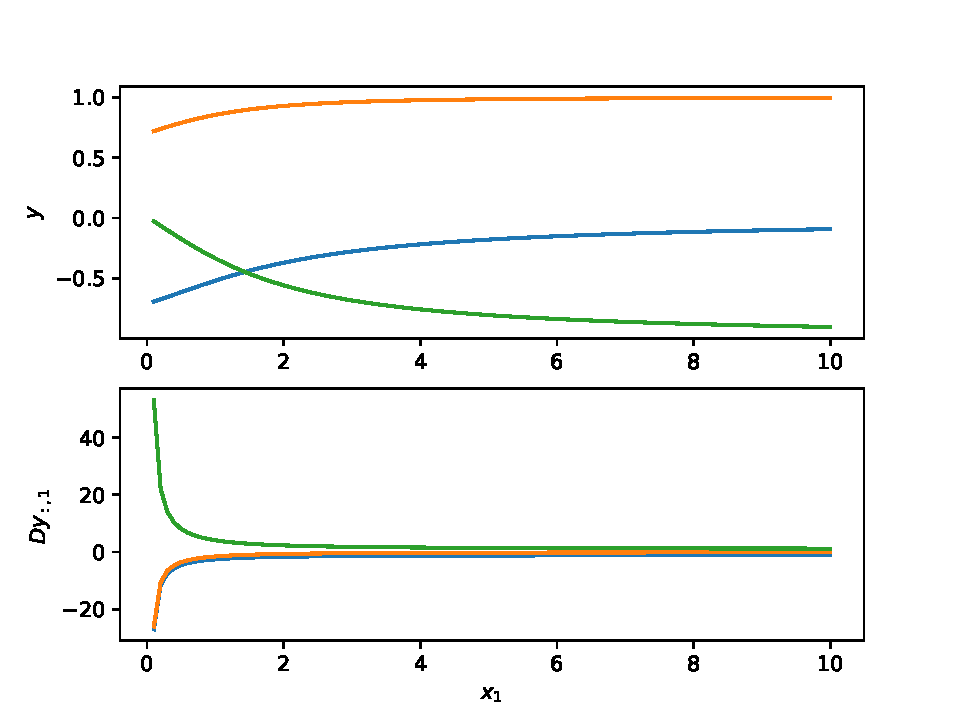
\includegraphics[page=1,width=.8\textwidth]{figs/multiple_inequality_example.pdf} 
    \caption{Plots of the function $y$ (top) and the gradient (bottom) sweeping the first component of the input $x_1$ while holding the other elements of $x$ constant}
\end{figure}
\par The deep declarative node is the instantiation of inequality constraints nodes with $n=3$ and $m=3$. Same as the feasible solution as the beginning, we set $x=\pi / 6$, which satisfies the inequality constraints since $\sin (\pi/6) < \cos (\pi/6)$. Figure~\ref{fig:ineq-eg} shows the function $y$ and its gradient changes. The gradient flattened to some extreme value at the beginning of the iteration then converge to almost zero. 

\section{Future Work of the Deep Declarative Network}
There are various possible challenging extensions of the deep declarative network in both theory and application. As a differentiable network, it combines the exact functionality solution with the iterative gradient method. In this section, we give several future foreseeable extensions of the declarative network comparing with other state-of-the-art differentiable models in both theory optimization and applications in computer vision tasks. 
\par We give the solution to the deep declarative nodes of constrained problems under the assumption that the solution of the problem $y(x)$ exists, and it should be a regular point whose gradient can be computed. Also, both objective function and constraints are required to be first and second-order differentiable, which also means that they are continuous instead of discrete. Therefore, in some computer vision tasks such as binary constrained classification problem may not be able to solve using this approach. Some relevant extension methods are discussed in PART II. Also, the robustness of the declarative nodes can be improved by introducing attention to specific constraints. 
\par In solving the real computer vision tasks, comparing to other differentiable models, the deep declarative network can be applied to the visual Sudoku problem. Also, many constrained optimization problems in the graph can be solved through this method. Future work in applications can focus on providing a more specific algorithm for different tasks. 

\section{Summary}
In Chapter~\ref{cha:ddn}, we describe the deep declarative network from its structure to its implementation with examples of different constrained problems. As a differentiable neural network, the deep declarative network defines its nodes to process input implicitly through the optimization problem, which can find the optimal solution directly without the verification of the local or global minimum. Its learning progress is also based on the derivative of the solution and the gradient of its constraints. We also introduce the back-propagation through deep declarative nodes in three subclasses: unconstrained, constrained, and inequality constrained problems. All representations of the gradient in declarative nodes have assumptions of the existence of the optimal point, its regularity, and its first and second-order derivative. In the next chapter, we are going to give an overview of the non-regular solution with related previous works. 